\documentclass{book}
\usepackage[a4paper,top=2.5cm,bottom=2.5cm,left=2.5cm,right=2.5cm]{geometry}
\usepackage{makeidx}
\usepackage{natbib}
\usepackage{graphicx}
\usepackage{multicol}
\usepackage{float}
\usepackage{listings}
\usepackage{color}
\usepackage{ifthen}
\usepackage[table]{xcolor}
\usepackage{textcomp}
\usepackage{alltt}
\usepackage{ifpdf}
\ifpdf
\usepackage[pdftex,
            pagebackref=true,
            colorlinks=true,
            linkcolor=blue,
            unicode
           ]{hyperref}
\else
\usepackage[ps2pdf,
            pagebackref=true,
            colorlinks=true,
            linkcolor=blue,
            unicode
           ]{hyperref}
\usepackage{pspicture}
\fi
\usepackage[utf8]{inputenc}
\usepackage[french]{babel}

\usepackage{mathptmx}
\usepackage[scaled=.90]{helvet}
\usepackage{courier}
\usepackage{sectsty}
\usepackage{amssymb}
\usepackage[titles]{tocloft}
\usepackage{doxygen}
\lstset{language=C++,inputencoding=utf8,basicstyle=\footnotesize,breaklines=true,breakatwhitespace=true,tabsize=8,numbers=left }
\makeindex
\setcounter{tocdepth}{3}
\renewcommand{\footrulewidth}{0.4pt}
\renewcommand{\familydefault}{\sfdefault}
\hfuzz=15pt
\setlength{\emergencystretch}{15pt}
\hbadness=750
\tolerance=750
\begin{document}
\hypersetup{pageanchor=false,citecolor=blue}
\begin{titlepage}
\vspace*{7cm}
\begin{center}
{\Large I\-G\-Osat Simulator }\\
\vspace*{1cm}
{\large Généré par Doxygen 1.8.1.2}\\
\vspace*{0.5cm}
{\small Mercredi Mars 5 2014 13:37:16}\\
\end{center}
\end{titlepage}
\clearemptydoublepage
\pagenumbering{roman}
\tableofcontents
\clearemptydoublepage
\pagenumbering{arabic}
\hypersetup{pageanchor=true,citecolor=blue}
\chapter{Liste des choses à faire}
\label{todo}
\hypertarget{todo}{}

\begin{DoxyRefList}
\item[\label{todo__todo000002}%
\hypertarget{todo__todo000002}{}%
Membre \hyperlink{classBatteryModule_a2fb494ef5f124c38c0fdf9ccfb31918f}{Battery\-Module\-:\-:Battery\-Module} (std\-::string name, Params params=Params())]Surcharger \mbox{[}\mbox{]} pour getsocketbyname  
\item[\label{todo__todo000004}%
\hypertarget{todo__todo000004}{}%
Classe \hyperlink{classISynchronized}{I\-Synchronized} ]Enventuellement factory de modules ?  
\item[\label{todo__todo000005}%
\hypertarget{todo__todo000005}{}%
Membre \hyperlink{classModule_ab7ea9648fa500696c85e93ebd0666390}{Module\-:\-:clock} (int)]Lever une exception  
\item[\label{todo__todo000006}%
\hypertarget{todo__todo000006}{}%
Membre \hyperlink{classModule_aed844ffed911793d3895c5a2bc4f9d43}{Module\-:\-:get\-Socket\-By\-Name} (std\-::string)]Faire le retour d'un objet 

Créer et gérer l'exception  
\item[\label{todo__todo000011}%
\hypertarget{todo__todo000011}{}%
Classe \hyperlink{classSocket}{Socket} ]Setconnection in \hyperlink{classSocket}{Socket} must be private and friend with Connection only !  
\item[\label{todo__todo000010}%
\hypertarget{todo__todo000010}{}%
Membre \hyperlink{classSocket_a71e162a0ca00b1a46fe23eaccb09f76d}{Socket\-:\-:get\-First\-Message} ()]Lever une exception  
\item[\label{todo__todo000009}%
\hypertarget{todo__todo000009}{}%
Membre \hyperlink{classSocket_a06b687baf9b01f3e399a5ee040ca04e4}{Socket\-:\-:send} (std\-::shared\-\_\-ptr$<$ Message $>$)]Et si connexion est null ? 
\end{DoxyRefList}
\chapter{Index des classes}
\section{Hiérarchie des classes}
Cette liste d'héritage est classée approximativement par ordre alphabétique \-:\begin{DoxyCompactList}
\item \contentsline{section}{Connexion}{\pageref{classConnexion}}{}
\item \contentsline{section}{H\-C\-I}{\pageref{classHCI}}{}
\begin{DoxyCompactList}
\item \contentsline{section}{C\-L\-I}{\pageref{classCLI}}{}
\item \contentsline{section}{File}{\pageref{classFile}}{}
\end{DoxyCompactList}
\item \contentsline{section}{H\-C\-Is}{\pageref{classHCIs}}{}
\item \contentsline{section}{I\-Synchronized}{\pageref{classISynchronized}}{}
\begin{DoxyCompactList}
\item \contentsline{section}{File}{\pageref{classFile}}{}
\item \contentsline{section}{Module}{\pageref{classModule}}{}
\begin{DoxyCompactList}
\item \contentsline{section}{Battery}{\pageref{classBattery}}{}
\item \contentsline{section}{Battery\-Controller}{\pageref{classBatteryController}}{}
\item \contentsline{section}{Macro\-Module}{\pageref{classMacroModule}}{}
\begin{DoxyCompactList}
\item \contentsline{section}{Battery\-Module}{\pageref{classBatteryModule}}{}
\end{DoxyCompactList}
\end{DoxyCompactList}
\item \contentsline{section}{Physics}{\pageref{classPhysics}}{}
\begin{DoxyCompactList}
\item \contentsline{section}{Battery\-Physics}{\pageref{classBatteryPhysics}}{}
\end{DoxyCompactList}
\item \contentsline{section}{Socket}{\pageref{classSocket}}{}
\end{DoxyCompactList}
\item \contentsline{section}{Memory$<$ T $>$}{\pageref{classMemory}}{}
\item \contentsline{section}{Message}{\pageref{classMessage}}{}
\begin{DoxyCompactList}
\item \contentsline{section}{Float\-Message}{\pageref{classFloatMessage}}{}
\item \contentsline{section}{Int\-Message}{\pageref{classIntMessage}}{}
\item \contentsline{section}{String\-Message}{\pageref{classStringMessage}}{}
\end{DoxyCompactList}
\item \contentsline{section}{Timer}{\pageref{classTimer}}{}
\item \contentsline{section}{X\-M\-L\-Reader}{\pageref{classXMLReader}}{}
\end{DoxyCompactList}

\chapter{Index des classes}
\section{Liste des classes}
Liste des classes, structures, unions et interfaces avec une brève description \-:\begin{DoxyCompactList}
\item\contentsline{section}{\hyperlink{classBattery}{Battery} }{\pageref{classBattery}}{}
\item\contentsline{section}{\hyperlink{classBatteryController}{Battery\-Controller} }{\pageref{classBatteryController}}{}
\item\contentsline{section}{\hyperlink{classBatteryModule}{Battery\-Module} \\*Un exemple de batterie }{\pageref{classBatteryModule}}{}
\item\contentsline{section}{\hyperlink{classBatteryPhysics}{Battery\-Physics} }{\pageref{classBatteryPhysics}}{}
\item\contentsline{section}{\hyperlink{classCLI}{C\-L\-I} \\*Implémentation de l'interface en ligne de commande (Command Line Interface) Sorties et entrées via la ligne de commande. Une seule instance possible de celle-\/ci, le pattern singleton a été utilisé }{\pageref{classCLI}}{}
\item\contentsline{section}{\hyperlink{classConnexion}{Connexion} \\*Cette classe représente les tuyaux qui relient les \hyperlink{classSocket}{Socket} }{\pageref{classConnexion}}{}
\item\contentsline{section}{\hyperlink{classFloatMessage}{Float\-Message} \\*Classe de messages contenant un nombre à virgule flottante comme le payload }{\pageref{classFloatMessage}}{}
\item\contentsline{section}{\hyperlink{classHCI}{H\-C\-I} \\*Classe d'abstraction pour l'interface utilisateur (Human Computer Interface) Cette interface vise abstraire les interactions avec l'utilisateur pour pouvoir ensutie \char`\"{}facilement\char`\"{} implémenter de nouvelles interfaces, graphiques notamment }{\pageref{classHCI}}{}
\item\contentsline{section}{\hyperlink{classIntMessage}{Int\-Message} \\*Classe de messages contenant entier comme le payload }{\pageref{classIntMessage}}{}
\item\contentsline{section}{\hyperlink{classISynchronized}{I\-Synchronized} \\*Interface pour élément synchronisé }{\pageref{classISynchronized}}{}
\item\contentsline{section}{\hyperlink{classMacroModule}{Macro\-Module} }{\pageref{classMacroModule}}{}
\item\contentsline{section}{\hyperlink{classMemory}{Memory$<$ T $>$} \\*Représente une mémoire }{\pageref{classMemory}}{}
\item\contentsline{section}{\hyperlink{classMessage}{Message} \\*Classe abstraite de base pour les messages }{\pageref{classMessage}}{}
\item\contentsline{section}{\hyperlink{classModule}{Module} \\*Les briques de base du simulateur }{\pageref{classModule}}{}
\item\contentsline{section}{\hyperlink{classPhysics}{Physics} \\*Classe abstraite pour décrire les différentes actions de l'environnement sur les modules }{\pageref{classPhysics}}{}
\item\contentsline{section}{\hyperlink{classSocket}{Socket} \\*Classe abstraite pour les connecteurs des modules }{\pageref{classSocket}}{}
\item\contentsline{section}{\hyperlink{classStringMessage}{String\-Message} \\*Classe de messages contenant une suite des caractères comme le payload }{\pageref{classStringMessage}}{}
\item\contentsline{section}{\hyperlink{classTimer}{Timer} \\*Cette classe sert à la gestion du temps simulé }{\pageref{classTimer}}{}
\item\contentsline{section}{\hyperlink{classXMLReader}{X\-M\-L\-Reader} \\*Classe utilitaire pour la lecture des fichiers de configuration }{\pageref{classXMLReader}}{}
\end{DoxyCompactList}

\chapter{Documentation des classes}
\hypertarget{classConnexion}{\section{Référence de la classe Connexion}
\label{classConnexion}\index{Connexion@{Connexion}}
}


Cette classe représente les tuyaux qui relient les \hyperlink{classSocket}{Socket}.  




{\ttfamily \#include $<$Connexion.\-h$>$}

\subsection*{Fonctions membres publiques}
\begin{DoxyCompactItemize}
\item 
\hyperlink{classConnexion_a31fda5acfafb5ec2de7ae76cfce373a7}{Connexion} (\hyperlink{classSocket}{Socket} $\ast$a, \hyperlink{classSocket}{Socket} $\ast$b)
\begin{DoxyCompactList}\small\item\em Constructeur, on créé une nouvelle connexion entre deux sockets en les informant mutuellement de leur compagnon (d'infortune ?). \end{DoxyCompactList}\item 
\hypertarget{classConnexion_a72dc9b8799eed7b02b7e75e8bccb601c}{{\bfseries Connexion} (const \hyperlink{classConnexion}{Connexion} \&)}\label{classConnexion_a72dc9b8799eed7b02b7e75e8bccb601c}

\item 
\hypertarget{classConnexion_a6afee761c33e160c2be5e9e2713968e3}{\hyperlink{classConnexion_a6afee761c33e160c2be5e9e2713968e3}{$\sim$\-Connexion} ()}\label{classConnexion_a6afee761c33e160c2be5e9e2713968e3}

\begin{DoxyCompactList}\small\item\em Destructeur. \end{DoxyCompactList}\item 
\hypertarget{classConnexion_ad39eca0322a2a8a49de21fdd910ea0db}{void \hyperlink{classConnexion_ad39eca0322a2a8a49de21fdd910ea0db}{dispatch} (std\-::shared\-\_\-ptr$<$ \hyperlink{classMessage}{Message} $>$, \hyperlink{classSocket}{Socket} $\ast$) const }\label{classConnexion_ad39eca0322a2a8a49de21fdd910ea0db}

\begin{DoxyCompactList}\small\item\em Envoie un message m d'un socket s vers son destinataire. \end{DoxyCompactList}\end{DoxyCompactItemize}


\subsection{Description détaillée}
Cette classe représente les tuyaux qui relient les \hyperlink{classSocket}{Socket}. 

\subsection{Documentation des constructeurs et destructeur}
\hypertarget{classConnexion_a31fda5acfafb5ec2de7ae76cfce373a7}{\index{Connexion@{Connexion}!Connexion@{Connexion}}
\index{Connexion@{Connexion}!Connexion@{Connexion}}
\subsubsection[{Connexion}]{\setlength{\rightskip}{0pt plus 5cm}Connexion\-::\-Connexion (
\begin{DoxyParamCaption}
\item[{{\bf Socket} $\ast$}]{a, }
\item[{{\bf Socket} $\ast$}]{b}
\end{DoxyParamCaption}
)}}\label{classConnexion_a31fda5acfafb5ec2de7ae76cfce373a7}


Constructeur, on créé une nouvelle connexion entre deux sockets en les informant mutuellement de leur compagnon (d'infortune ?). 

Constructeurpar copie. 

La documentation de cette classe a été générée à partir des fichiers suivants \-:\begin{DoxyCompactItemize}
\item 
src/\-Core/Connexion.\-h\item 
src/\-Core/Connexion.\-cpp\end{DoxyCompactItemize}

\hypertarget{classMacroModule}{\section{Référence de la classe Macro\-Module}
\label{classMacroModule}\index{Macro\-Module@{Macro\-Module}}
}
Graphe d'héritage de Macro\-Module\-:\begin{figure}[H]
\begin{center}
\leavevmode
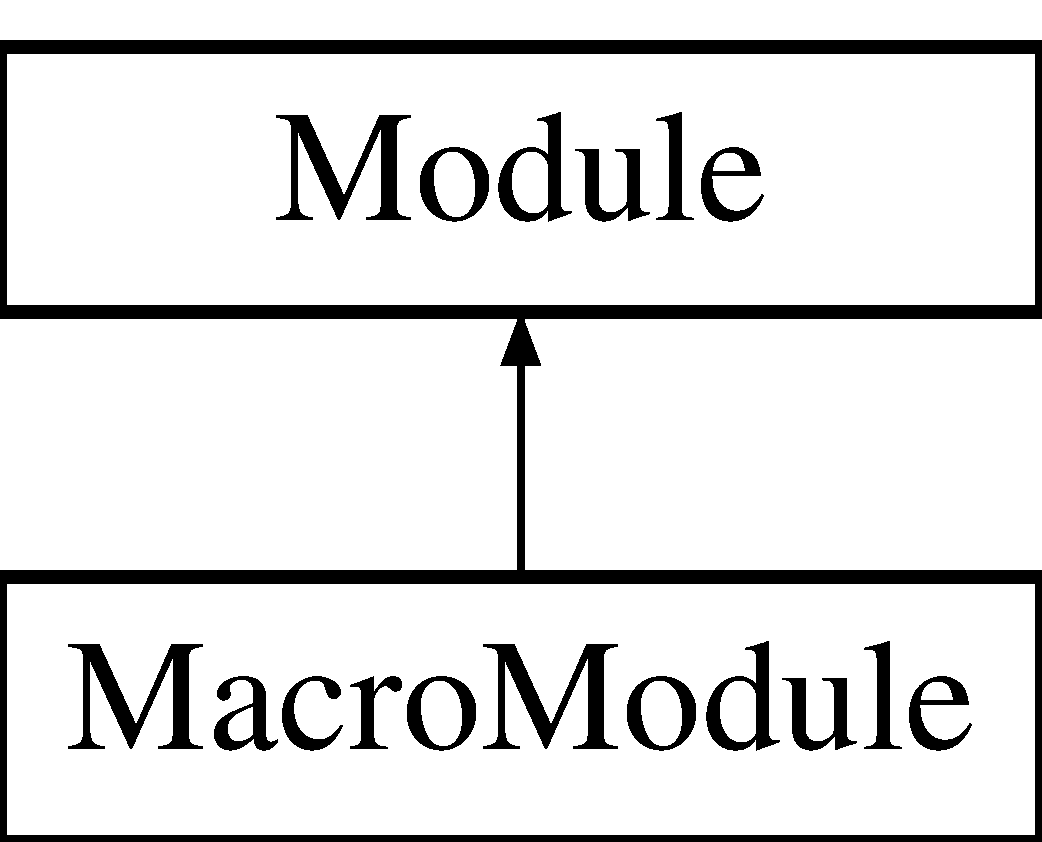
\includegraphics[height=4.000000cm]{classMacroModule}
\end{center}
\end{figure}
\subsection*{Fonctions membres publiques}
\begin{DoxyCompactItemize}
\item 
\hypertarget{classMacroModule_a9a7fef08bb03b97cb018b4cd7ad95c64}{{\bfseries Macro\-Module} (std\-::string=\char`\"{}Default\-Name\char`\"{}, Params=Params(), std\-::string cp=std\-::string())}\label{classMacroModule_a9a7fef08bb03b97cb018b4cd7ad95c64}

\item 
\hypertarget{classMacroModule_aa7d592010b740d68028fee87e139ae9f}{\hyperlink{classMacroModule_aa7d592010b740d68028fee87e139ae9f}{Macro\-Module} (std\-::string, \hyperlink{classMemory}{Memory}$<$ int $>$, Params=Params())}\label{classMacroModule_aa7d592010b740d68028fee87e139ae9f}

\begin{DoxyCompactList}\small\item\em Constructeur avec m�moire. \end{DoxyCompactList}\item 
\hypertarget{classMacroModule_a9790fb7c331d99dd03f624b1a5258519}{virtual \hyperlink{classMacroModule_a9790fb7c331d99dd03f624b1a5258519}{$\sim$\-Macro\-Module} ()}\label{classMacroModule_a9790fb7c331d99dd03f624b1a5258519}

\begin{DoxyCompactList}\small\item\em Destructeur. \end{DoxyCompactList}\item 
\hypertarget{classMacroModule_a3c693014fb5e1a46758e7867eca43342}{void \hyperlink{classMacroModule_a3c693014fb5e1a46758e7867eca43342}{add\-Sub\-Module} (\hyperlink{classModule}{Module} $\ast$)}\label{classMacroModule_a3c693014fb5e1a46758e7867eca43342}

\begin{DoxyCompactList}\small\item\em Ajoute un sous-\/module � la liste. \end{DoxyCompactList}\item 
\hypertarget{classMacroModule_a6ad4d6abd8bb4b742b800f6fa3c98296}{void \hyperlink{classMacroModule_a6ad4d6abd8bb4b742b800f6fa3c98296}{add\-Connexion} (\hyperlink{classConnexion}{Connexion} $\ast$)}\label{classMacroModule_a6ad4d6abd8bb4b742b800f6fa3c98296}

\begin{DoxyCompactList}\small\item\em Ajoute une connexion � la liste. \end{DoxyCompactList}\item 
\hypertarget{classMacroModule_ab98b15af55e4cd1ad3a20fc53af09aa4}{std\-::shared\-\_\-ptr$<$ \hyperlink{classModule}{Module} $>$ \hyperlink{classMacroModule_ab98b15af55e4cd1ad3a20fc53af09aa4}{get\-Module\-By\-Name} (std\-::string)}\label{classMacroModule_ab98b15af55e4cd1ad3a20fc53af09aa4}

\begin{DoxyCompactList}\small\item\em Renvoie le module voulu Exception g�r�e. \end{DoxyCompactList}\end{DoxyCompactItemize}
\subsection*{Additional Inherited Members}


La documentation de cette classe a été générée à partir des fichiers suivants \-:\begin{DoxyCompactItemize}
\item 
src/\-Core/Macro\-Module.\-h\item 
src/\-Core/Macro\-Module.\-cpp\end{DoxyCompactItemize}

\hypertarget{classMemory}{\section{Référence du modèle de la classe Memory$<$ T $>$}
\label{classMemory}\index{Memory$<$ T $>$@{Memory$<$ T $>$}}
}


Représente une mémoire.  




{\ttfamily \#include $<$Memory.\-h$>$}

\subsection*{Fonctions membres publiques}
\begin{DoxyCompactItemize}
\item 
\hypertarget{classMemory_aa546b7c6e170e45a4e4f74492d8fe8bf}{\hyperlink{classMemory_aa546b7c6e170e45a4e4f74492d8fe8bf}{Memory} ()}\label{classMemory_aa546b7c6e170e45a4e4f74492d8fe8bf}

\begin{DoxyCompactList}\small\item\em Constructeur. \end{DoxyCompactList}\item 
\hypertarget{classMemory_af1e6452dbe3bb1650604140814710b95}{\hyperlink{classMemory_af1e6452dbe3bb1650604140814710b95}{Memory} (std\-::unordered\-\_\-map$<$ std\-::string, T $>$)}\label{classMemory_af1e6452dbe3bb1650604140814710b95}

\begin{DoxyCompactList}\small\item\em Constructeur parametrisé avec cells. \end{DoxyCompactList}\item 
\hypertarget{classMemory_add46d3ed56cf1e88efee2ed59b38c995}{unsigned int \hyperlink{classMemory_add46d3ed56cf1e88efee2ed59b38c995}{get\-Size} ()}\label{classMemory_add46d3ed56cf1e88efee2ed59b38c995}

\begin{DoxyCompactList}\small\item\em Retourne la taille courante de la mémoire. \end{DoxyCompactList}\item 
\hypertarget{classMemory_a3514e7594615bb1748ba5b57259c9eca}{int \hyperlink{classMemory_a3514e7594615bb1748ba5b57259c9eca}{set\-Value\-For\-Key} (std\-::string, T)}\label{classMemory_a3514e7594615bb1748ba5b57259c9eca}

\begin{DoxyCompactList}\small\item\em écrit une valeur \char`\"{}value\char`\"{} dans la case mémoire avec un nom \char`\"{}key\char`\"{}. \end{DoxyCompactList}\item 
\hypertarget{classMemory_a2d153fdede89954dc0875ab6c8d804c3}{\hyperlink{classMemory_a2d153fdede89954dc0875ab6c8d804c3}{$\sim$\-Memory} ()}\label{classMemory_a2d153fdede89954dc0875ab6c8d804c3}

\begin{DoxyCompactList}\small\item\em Destructeur. \end{DoxyCompactList}\end{DoxyCompactItemize}


\subsection{Description détaillée}
\subsubsection*{template$<$class T$>$class Memory$<$ T $>$}

Représente une mémoire. 

La mémoire est ici simplement modélisée comme une liste de clées et de valeurs, associée à des contraintes. 

La documentation de cette classe a été générée à partir des fichiers suivants \-:\begin{DoxyCompactItemize}
\item 
src/\-Core/Memory.\-h\item 
src/\-Core/Memory.\-cpp\end{DoxyCompactItemize}

\hypertarget{classMessage}{\section{Référence de la classe Message}
\label{classMessage}\index{Message@{Message}}
}


Classe abstraite de base pour les messages.  




{\ttfamily \#include $<$Message.\-h$>$}

Graphe d'héritage de Message\-:\begin{figure}[H]
\begin{center}
\leavevmode
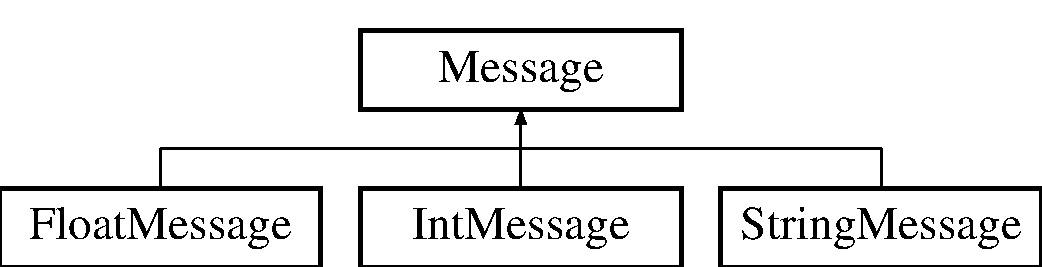
\includegraphics[height=2.000000cm]{classMessage}
\end{center}
\end{figure}
\subsection*{Fonctions membres publiques}
\begin{DoxyCompactItemize}
\item 
\hypertarget{classMessage_a154809183fa5ec6b5182c487db1167dd}{\hyperlink{classMessage_a154809183fa5ec6b5182c487db1167dd}{Message} (std\-::string \hyperlink{classMessage_ac7adddb666acdc47c48f684bd6810a51}{name}=\char`\"{}Default Name\char`\"{}, int=0)}\label{classMessage_a154809183fa5ec6b5182c487db1167dd}

\begin{DoxyCompactList}\small\item\em Constructeur par défaut. \end{DoxyCompactList}\item 
\hypertarget{classMessage_a3f7275462831f787a861271687bcad67}{virtual \hyperlink{classMessage_a3f7275462831f787a861271687bcad67}{$\sim$\-Message} ()}\label{classMessage_a3f7275462831f787a861271687bcad67}

\begin{DoxyCompactList}\small\item\em Destructeur. \end{DoxyCompactList}\item 
\hypertarget{classMessage_ac03b02000572b0852c574498bf138e87}{std\-::string \hyperlink{classMessage_ac03b02000572b0852c574498bf138e87}{get\-Name} ()}\label{classMessage_ac03b02000572b0852c574498bf138e87}

\begin{DoxyCompactList}\small\item\em Renvoie le nom du message. \end{DoxyCompactList}\item 
\hypertarget{classMessage_acbdab136245666bce3752fa311150672}{virtual std\-::ostream \& \hyperlink{classMessage_acbdab136245666bce3752fa311150672}{operator$<$$<$} (std\-::ostream \&os)=0}\label{classMessage_acbdab136245666bce3752fa311150672}

\begin{DoxyCompactList}\small\item\em Operateur de sortie surchargé \end{DoxyCompactList}\item 
\hypertarget{classMessage_a37550fee6e64d7c83ead2628373f4db3}{unsigned int \hyperlink{classMessage_a37550fee6e64d7c83ead2628373f4db3}{get\-Transmission\-Time} ()}\label{classMessage_a37550fee6e64d7c83ead2628373f4db3}

\begin{DoxyCompactList}\small\item\em Renvoie le temps de traitement du message. \end{DoxyCompactList}\end{DoxyCompactItemize}
\subsection*{Fonctions membres publiques statiques}
\begin{DoxyCompactItemize}
\item 
\hypertarget{classMessage_a18fddc1357914aa65d4a12eeabbf7bfa}{static std\-::shared\-\_\-ptr$<$ \hyperlink{classMessage}{Message} $>$ {\bfseries create\-Message} (std\-::string, int=0, unsigned int=0)}\label{classMessage_a18fddc1357914aa65d4a12eeabbf7bfa}

\item 
\hypertarget{classMessage_a9510bbfbcde96a857eb40b8222fe90a8}{static std\-::shared\-\_\-ptr$<$ \hyperlink{classMessage}{Message} $>$ {\bfseries create\-Message} (std\-::string, std\-::string=\char`\"{}\char`\"{}, unsigned int=0)}\label{classMessage_a9510bbfbcde96a857eb40b8222fe90a8}

\item 
\hypertarget{classMessage_a275c24aa740943af5872d874eeca0173}{static std\-::shared\-\_\-ptr$<$ \hyperlink{classMessage}{Message} $>$ \hyperlink{classMessage_a275c24aa740943af5872d874eeca0173}{create\-Message} (std\-::string, float=0, unsigned=0)}\label{classMessage_a275c24aa740943af5872d874eeca0173}

\begin{DoxyCompactList}\small\item\em Crée et retourne le pointeur partagé au nouveau \hyperlink{classFloatMessage}{Float\-Message}. \end{DoxyCompactList}\end{DoxyCompactItemize}
\subsection*{Attributs protégés}
\begin{DoxyCompactItemize}
\item 
std\-::string \hyperlink{classMessage_ac7adddb666acdc47c48f684bd6810a51}{name}
\item 
unsigned int \hyperlink{classMessage_a9f2d70860e0ec546c8e00cd69a3555ee}{transmission\-Time}
\end{DoxyCompactItemize}


\subsection{Description détaillée}
Classe abstraite de base pour les messages. 

Les messages sont les différentes informations que peuvent se communiquer les modules. Un message est composé de son nom, éventuellement d'une donnée (payload), et d'une indication temporelle concernant la durée de son envoi et de sa réception. 

\subsection{Documentation des données membres}
\hypertarget{classMessage_ac7adddb666acdc47c48f684bd6810a51}{\index{Message@{Message}!name@{name}}
\index{name@{name}!Message@{Message}}
\subsubsection[{name}]{\setlength{\rightskip}{0pt plus 5cm}std\-::string Message\-::name\hspace{0.3cm}{\ttfamily [protected]}}}\label{classMessage_ac7adddb666acdc47c48f684bd6810a51}
Nom du message \hypertarget{classMessage_a9f2d70860e0ec546c8e00cd69a3555ee}{\index{Message@{Message}!transmission\-Time@{transmission\-Time}}
\index{transmission\-Time@{transmission\-Time}!Message@{Message}}
\subsubsection[{transmission\-Time}]{\setlength{\rightskip}{0pt plus 5cm}unsigned int Message\-::transmission\-Time\hspace{0.3cm}{\ttfamily [protected]}}}\label{classMessage_a9f2d70860e0ec546c8e00cd69a3555ee}
Temps de traitement du message 

La documentation de cette classe a été générée à partir des fichiers suivants \-:\begin{DoxyCompactItemize}
\item 
src/\-Core/Message.\-h\item 
src/\-Core/Message.\-cpp\end{DoxyCompactItemize}

\hypertarget{classModule}{\section{Référence de la classe Module}
\label{classModule}\index{Module@{Module}}
}


Les briques de base du simulateur.  




{\ttfamily \#include $<$Module.\-h$>$}

Graphe d'héritage de Module\-:\begin{figure}[H]
\begin{center}
\leavevmode
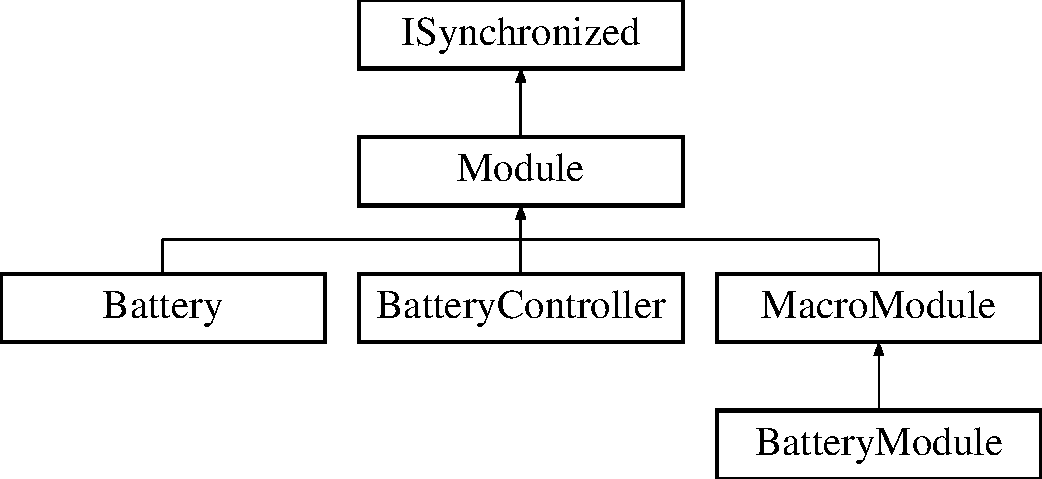
\includegraphics[height=4.000000cm]{classModule}
\end{center}
\end{figure}
\subsection*{Fonctions membres publiques}
\begin{DoxyCompactItemize}
\item 
\hypertarget{classModule_abcdd948c7444d3420f04be1bd332fbae}{\hyperlink{classModule_abcdd948c7444d3420f04be1bd332fbae}{Module} (std\-::string=\char`\"{}Default\-Name\char`\"{}, Params=Params(), std\-::string cp=std\-::string())}\label{classModule_abcdd948c7444d3420f04be1bd332fbae}

\begin{DoxyCompactList}\small\item\em Constructeur par défault, pour un module sans mémoire. \end{DoxyCompactList}\item 
\hypertarget{classModule_ae2ce24f11deec1453dfaba1f21a36f2c}{\hyperlink{classModule_ae2ce24f11deec1453dfaba1f21a36f2c}{Module} (std\-::string, \hyperlink{classMemory}{Memory}$<$ int $>$, Params=Params())}\label{classModule_ae2ce24f11deec1453dfaba1f21a36f2c}

\begin{DoxyCompactList}\small\item\em Constructeur avec mémoire. \end{DoxyCompactList}\item 
\hypertarget{classModule_a7c9d9c096786d127590fdd8aa2b7d681}{virtual \hyperlink{classModule_a7c9d9c096786d127590fdd8aa2b7d681}{$\sim$\-Module} ()}\label{classModule_a7c9d9c096786d127590fdd8aa2b7d681}

\begin{DoxyCompactList}\small\item\em Destructeur. \end{DoxyCompactList}\item 
virtual void \hyperlink{classModule_ab7ea9648fa500696c85e93ebd0666390}{clock} (int)
\begin{DoxyCompactList}\small\item\em Méthode appellée à chaque pas de temps, commune à tous les modules. \end{DoxyCompactList}\item 
\hypertarget{classModule_aeb7302c667eb923a4dc25ae235c744dc}{void \hyperlink{classModule_aeb7302c667eb923a4dc25ae235c744dc}{add\-Socket} (\hyperlink{classSocket}{Socket})}\label{classModule_aeb7302c667eb923a4dc25ae235c744dc}

\begin{DoxyCompactList}\small\item\em Fonction d'ajout d'un connecteur au module. \end{DoxyCompactList}\item 
\hypertarget{classModule_a146f454fded03cda14359e419086afa5}{void \hyperlink{classModule_a146f454fded03cda14359e419086afa5}{add\-Message} (std\-::string, int)}\label{classModule_a146f454fded03cda14359e419086afa5}

\begin{DoxyCompactList}\small\item\em Fonction d'ajout d'un message au module, et de son temps d'éxecution simulé. \end{DoxyCompactList}\item 
\hyperlink{classSocket}{Socket} $\ast$ \hyperlink{classModule_aed844ffed911793d3895c5a2bc4f9d43}{get\-Socket\-By\-Name} (std\-::string)
\begin{DoxyCompactList}\small\item\em Récupère le bon connecteur, ou lève une exception. \end{DoxyCompactList}\item 
\hypertarget{classModule_a93e2ee84587751939c1fd31cb0802e41}{double {\bfseries get\-Param\-Value\-By\-Name} (std\-::string)}\label{classModule_a93e2ee84587751939c1fd31cb0802e41}

\item 
\hypertarget{classModule_ace0e4299e1a6f9b46aa9fd316483895d}{void {\bfseries set\-Param\-Value\-By\-Name} (std\-::string, double)}\label{classModule_ace0e4299e1a6f9b46aa9fd316483895d}

\item 
\hypertarget{classModule_a6e425394cec58009568822cc7a09c8c1}{bool \hyperlink{classModule_a6e425394cec58009568822cc7a09c8c1}{is\-Message\-Allowed} (std\-::string)}\label{classModule_a6e425394cec58009568822cc7a09c8c1}

\begin{DoxyCompactList}\small\item\em Vérifie si le message est un des messages compris par ce module. \end{DoxyCompactList}\item 
\hypertarget{classModule_a3c1ecab9c7fa778807e253c26aa54310}{std\-::string \hyperlink{classModule_a3c1ecab9c7fa778807e253c26aa54310}{get\-Name} () const }\label{classModule_a3c1ecab9c7fa778807e253c26aa54310}

\begin{DoxyCompactList}\small\item\em Vérifie si le message est un des messages compris par ce module. \end{DoxyCompactList}\end{DoxyCompactItemize}
\subsection*{Attributs protégés}
\begin{DoxyCompactItemize}
\item 
std\-::string \hyperlink{classModule_a794fbb44972c7c73cc197159093e66d1}{name}
\item 
std\-::string \hyperlink{classModule_a5c7481c5ac746e01b225b6782e915dac}{conf\-Path}
\item 
\hyperlink{classMemory}{Memory}$<$ int $>$ \hyperlink{classModule_a48fa02fe55d33daffff725c615a63bb9}{memory}
\item 
Sockets \hyperlink{classModule_af0415ddaab230958f91665c66b078085}{sockets}
\item 
Messages \hyperlink{classModule_aaadd1f971bebf7bb5eae12fcc5689198}{messages\-Allowed}
\item 
Params \hyperlink{classModule_a232443111a9d59c17724992ddf75fbad}{parameters}
\item 
std\-::queue$<$ std\-::shared\-\_\-ptr\\*
$<$ \hyperlink{classMessage}{Message} $>$ $>$ \hyperlink{classModule_a93e833bd46e53a2d52ab63afb304b840}{tasks}
\item 
int \hyperlink{classModule_afc209c4f9120425219f7775c79cf4bea}{task\-Timer}
\end{DoxyCompactItemize}


\subsection{Description détaillée}
Les briques de base du simulateur. 

Il s'agit de la classe centrale du simulateur, qui sera construit comme un assemblage de modules qui communiquent entre eux. Il s'agit d'une classe virtuelle. Nécessitant un contrôle de la part du timer, elle implémente l'interface \hyperlink{classISynchronized}{I\-Synchronized} 

\subsection{Documentation des fonctions membres}
\hypertarget{classModule_ab7ea9648fa500696c85e93ebd0666390}{\index{Module@{Module}!clock@{clock}}
\index{clock@{clock}!Module@{Module}}
\subsubsection[{clock}]{\setlength{\rightskip}{0pt plus 5cm}void Module\-::clock (
\begin{DoxyParamCaption}
\item[{int}]{time}
\end{DoxyParamCaption}
)\hspace{0.3cm}{\ttfamily [virtual]}}}\label{classModule_ab7ea9648fa500696c85e93ebd0666390}


Méthode appellée à chaque pas de temps, commune à tous les modules. 

Cette méthode effectue trois actions, lire les messages arrivés, avancer dans un processus interne, envoyer un message. Ces actions prennent tous du temps\-: elles peuvent durer plusieurs \char`\"{}ticks\char`\"{}. \begin{DoxyRefDesc}{A faire}
\item[\hyperlink{todo__todo000005}{A faire}]Lever une exception \end{DoxyRefDesc}


Implémente \hyperlink{classISynchronized_af7155c662758d6c70f381bb9b11afcd6}{I\-Synchronized}.

\hypertarget{classModule_aed844ffed911793d3895c5a2bc4f9d43}{\index{Module@{Module}!get\-Socket\-By\-Name@{get\-Socket\-By\-Name}}
\index{get\-Socket\-By\-Name@{get\-Socket\-By\-Name}!Module@{Module}}
\subsubsection[{get\-Socket\-By\-Name}]{\setlength{\rightskip}{0pt plus 5cm}{\bf Socket} $\ast$ Module\-::get\-Socket\-By\-Name (
\begin{DoxyParamCaption}
\item[{std\-::string}]{}
\end{DoxyParamCaption}
)}}\label{classModule_aed844ffed911793d3895c5a2bc4f9d43}


Récupère le bon connecteur, ou lève une exception. 

\begin{DoxyRefDesc}{A faire}
\item[\hyperlink{todo__todo000007}{A faire}]Créer et gérer l'exception \end{DoxyRefDesc}
\begin{DoxyRefDesc}{A faire}
\item[\hyperlink{todo__todo000006}{A faire}]Faire le retour d'un objet \end{DoxyRefDesc}


\subsection{Documentation des données membres}
\hypertarget{classModule_a5c7481c5ac746e01b225b6782e915dac}{\index{Module@{Module}!conf\-Path@{conf\-Path}}
\index{conf\-Path@{conf\-Path}!Module@{Module}}
\subsubsection[{conf\-Path}]{\setlength{\rightskip}{0pt plus 5cm}std\-::string Module\-::conf\-Path\hspace{0.3cm}{\ttfamily [protected]}}}\label{classModule_a5c7481c5ac746e01b225b6782e915dac}
Le chemin vers le fichier de configuration \hypertarget{classModule_a48fa02fe55d33daffff725c615a63bb9}{\index{Module@{Module}!memory@{memory}}
\index{memory@{memory}!Module@{Module}}
\subsubsection[{memory}]{\setlength{\rightskip}{0pt plus 5cm}{\bf Memory}$<$int$>$ Module\-::memory\hspace{0.3cm}{\ttfamily [protected]}}}\label{classModule_a48fa02fe55d33daffff725c615a63bb9}
La mémoire du module \hypertarget{classModule_aaadd1f971bebf7bb5eae12fcc5689198}{\index{Module@{Module}!messages\-Allowed@{messages\-Allowed}}
\index{messages\-Allowed@{messages\-Allowed}!Module@{Module}}
\subsubsection[{messages\-Allowed}]{\setlength{\rightskip}{0pt plus 5cm}Messages Module\-::messages\-Allowed\hspace{0.3cm}{\ttfamily [protected]}}}\label{classModule_aaadd1f971bebf7bb5eae12fcc5689198}
Les messages compris par le module E\-T leurs temps d'éxecution \hypertarget{classModule_a794fbb44972c7c73cc197159093e66d1}{\index{Module@{Module}!name@{name}}
\index{name@{name}!Module@{Module}}
\subsubsection[{name}]{\setlength{\rightskip}{0pt plus 5cm}std\-::string Module\-::name\hspace{0.3cm}{\ttfamily [protected]}}}\label{classModule_a794fbb44972c7c73cc197159093e66d1}
Le nom du module \hypertarget{classModule_a232443111a9d59c17724992ddf75fbad}{\index{Module@{Module}!parameters@{parameters}}
\index{parameters@{parameters}!Module@{Module}}
\subsubsection[{parameters}]{\setlength{\rightskip}{0pt plus 5cm}Params Module\-::parameters\hspace{0.3cm}{\ttfamily [protected]}}}\label{classModule_a232443111a9d59c17724992ddf75fbad}
Les paramètres d'état du modules \hypertarget{classModule_af0415ddaab230958f91665c66b078085}{\index{Module@{Module}!sockets@{sockets}}
\index{sockets@{sockets}!Module@{Module}}
\subsubsection[{sockets}]{\setlength{\rightskip}{0pt plus 5cm}Sockets Module\-::sockets\hspace{0.3cm}{\ttfamily [protected]}}}\label{classModule_af0415ddaab230958f91665c66b078085}
Les connecteurs du module \hypertarget{classModule_a93e833bd46e53a2d52ab63afb304b840}{\index{Module@{Module}!tasks@{tasks}}
\index{tasks@{tasks}!Module@{Module}}
\subsubsection[{tasks}]{\setlength{\rightskip}{0pt plus 5cm}std\-::queue$<$std\-::shared\-\_\-ptr$<${\bf Message}$>$ $>$ Module\-::tasks\hspace{0.3cm}{\ttfamily [protected]}}}\label{classModule_a93e833bd46e53a2d52ab63afb304b840}
La file d'attente des messages à traiter \hypertarget{classModule_afc209c4f9120425219f7775c79cf4bea}{\index{Module@{Module}!task\-Timer@{task\-Timer}}
\index{task\-Timer@{task\-Timer}!Module@{Module}}
\subsubsection[{task\-Timer}]{\setlength{\rightskip}{0pt plus 5cm}int Module\-::task\-Timer\hspace{0.3cm}{\ttfamily [protected]}}}\label{classModule_afc209c4f9120425219f7775c79cf4bea}
Le timer de la tâche courante 

La documentation de cette classe a été générée à partir des fichiers suivants \-:\begin{DoxyCompactItemize}
\item 
src/\-Core/Module.\-h\item 
src/\-Core/Module.\-cpp\end{DoxyCompactItemize}

\hypertarget{classNumberGeneratorModule}{\section{Référence de la classe Number\-Generator\-Module}
\label{classNumberGeneratorModule}\index{Number\-Generator\-Module@{Number\-Generator\-Module}}
}
Graphe d'héritage de Number\-Generator\-Module\-:\begin{figure}[H]
\begin{center}
\leavevmode
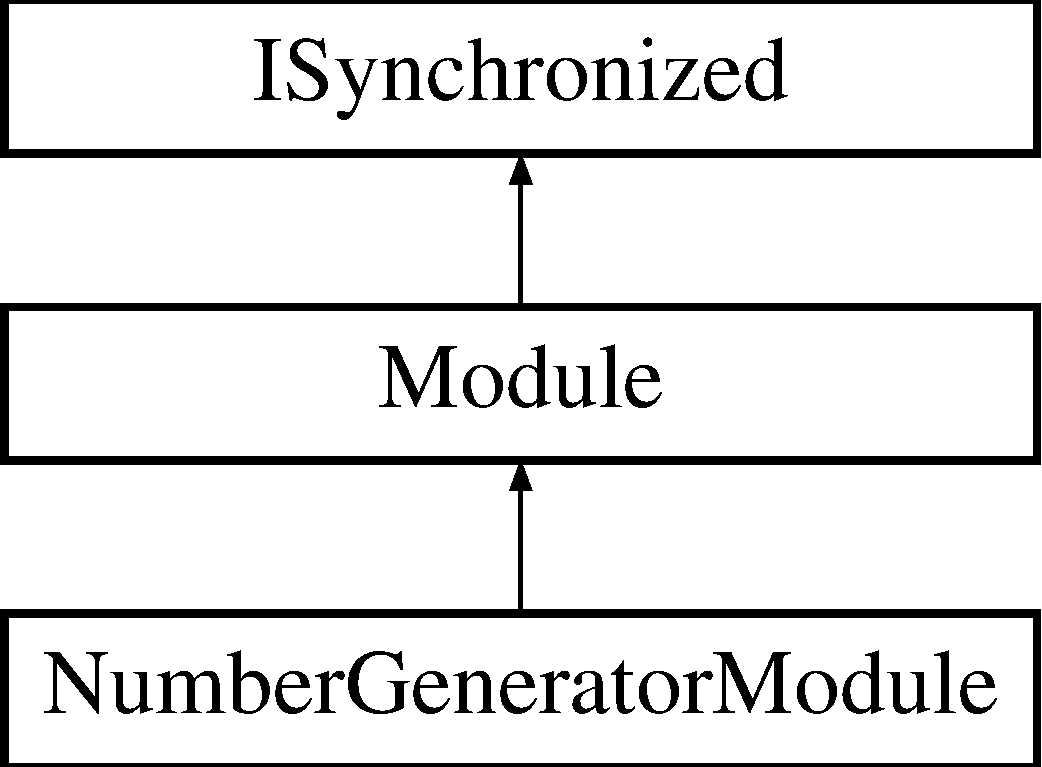
\includegraphics[height=3.000000cm]{classNumberGeneratorModule}
\end{center}
\end{figure}
\subsection*{Fonctions membres publiques}
\begin{DoxyCompactItemize}
\item 
\hypertarget{classNumberGeneratorModule_a92587409c57409b1aae930e37273959d}{void {\bfseries start} ()}\label{classNumberGeneratorModule_a92587409c57409b1aae930e37273959d}

\item 
\hypertarget{classNumberGeneratorModule_ae6d73ee8e66db56e83b01e86b70db9c1}{\hyperlink{classSocket}{Socket} $\ast$ {\bfseries get\-Out\-Socket} ()}\label{classNumberGeneratorModule_ae6d73ee8e66db56e83b01e86b70db9c1}

\end{DoxyCompactItemize}
\subsection*{Additional Inherited Members}


La documentation de cette classe a été générée à partir des fichiers suivants \-:\begin{DoxyCompactItemize}
\item 
src/headers/Number\-Generator\-Module.\-h\item 
src/includes/Number\-Generator\-Module.\-cpp\end{DoxyCompactItemize}

\hypertarget{classSocket}{\section{Référence de la classe Socket}
\label{classSocket}\index{Socket@{Socket}}
}


Classe abstraite pour les connecteurs des modules.  




{\ttfamily \#include $<$Socket.\-h$>$}

Graphe d'héritage de Socket\-:\begin{figure}[H]
\begin{center}
\leavevmode
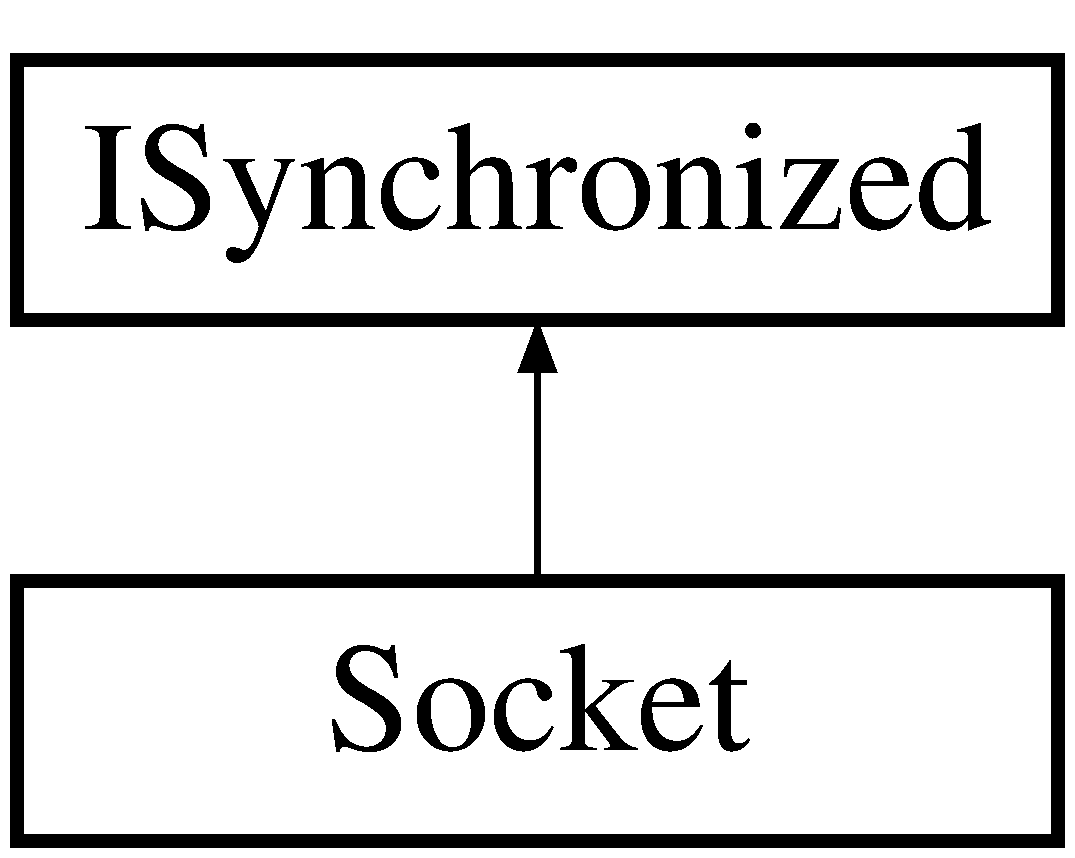
\includegraphics[height=2.000000cm]{classSocket}
\end{center}
\end{figure}
\subsection*{Fonctions membres publiques}
\begin{DoxyCompactItemize}
\item 
\hypertarget{classSocket_a0365662f7a20fa1cc6ef54fd2a659cfc}{{\bfseries Socket} (std\-::string name=\char`\"{}Socket\-Name\char`\"{}, std\-::string owner=\char`\"{}Socket\-Owner\char`\"{})}\label{classSocket_a0365662f7a20fa1cc6ef54fd2a659cfc}

\item 
\hypertarget{classSocket_a0dd97f1387c3bd8008cb7de47583a985}{{\bfseries Socket} (const \hyperlink{classSocket}{Socket} \&)}\label{classSocket_a0dd97f1387c3bd8008cb7de47583a985}

\item 
\hypertarget{classSocket_aeac4eb6379a543d38ed88977d3b6630a}{\hyperlink{classSocket_aeac4eb6379a543d38ed88977d3b6630a}{$\sim$\-Socket} ()}\label{classSocket_aeac4eb6379a543d38ed88977d3b6630a}

\begin{DoxyCompactList}\small\item\em Destructeur. \end{DoxyCompactList}\item 
\hypertarget{classSocket_a96d104e32d5f376796fb411874954e7d}{void \hyperlink{classSocket_a96d104e32d5f376796fb411874954e7d}{set\-Connexion} (\hyperlink{classConnexion}{Connexion} \&c)}\label{classSocket_a96d104e32d5f376796fb411874954e7d}

\begin{DoxyCompactList}\small\item\em Branche le socket à la connexion c. \end{DoxyCompactList}\item 
\hypertarget{classSocket_aaefa10006cbf7a7a082e4adc606b3cea}{std\-::string \hyperlink{classSocket_aaefa10006cbf7a7a082e4adc606b3cea}{get\-Name} ()}\label{classSocket_aaefa10006cbf7a7a082e4adc606b3cea}

\begin{DoxyCompactList}\small\item\em Retourne le nom de socket. \end{DoxyCompactList}\item 
\hypertarget{classSocket_a6421574ae64f7b40e7c3f7bbb5cc3cee}{std\-::string \hyperlink{classSocket_a6421574ae64f7b40e7c3f7bbb5cc3cee}{get\-Owner} ()}\label{classSocket_a6421574ae64f7b40e7c3f7bbb5cc3cee}

\begin{DoxyCompactList}\small\item\em Retourne le nom de module qui possede ce socket. \end{DoxyCompactList}\item 
\hypertarget{classSocket_a9adf799b90c455f3a1f4151adb031fd0}{void \hyperlink{classSocket_a9adf799b90c455f3a1f4151adb031fd0}{receive} (std\-::shared\-\_\-ptr$<$ \hyperlink{classMessage}{Message} $>$)}\label{classSocket_a9adf799b90c455f3a1f4151adb031fd0}

\begin{DoxyCompactList}\small\item\em Met le message m dans la file d'attente de socket. \end{DoxyCompactList}\item 
void \hyperlink{classSocket_a06b687baf9b01f3e399a5ee040ca04e4}{send} (std\-::shared\-\_\-ptr$<$ \hyperlink{classMessage}{Message} $>$)
\begin{DoxyCompactList}\small\item\em Envoye. \end{DoxyCompactList}\item 
\hypertarget{classSocket_a6bd5bddfabd838a3388b445c21d3c41e}{virtual void \hyperlink{classSocket_a6bd5bddfabd838a3388b445c21d3c41e}{clock} (int time)}\label{classSocket_a6bd5bddfabd838a3388b445c21d3c41e}

\begin{DoxyCompactList}\small\item\em Methode appellé à chaque tick d'horloge liée. \end{DoxyCompactList}\item 
\hypertarget{classSocket_afe7c9b2ef7fb3653b14f5f462293549a}{bool {\bfseries has\-Message} ()}\label{classSocket_afe7c9b2ef7fb3653b14f5f462293549a}

\item 
std\-::shared\-\_\-ptr$<$ \hyperlink{classMessage}{Message} $>$ \hyperlink{classSocket_a71e162a0ca00b1a46fe23eaccb09f76d}{get\-First\-Message} ()
\item 
\hypertarget{classSocket_aa890633022a29b56ed3844684d32e0fc}{int \hyperlink{classSocket_aa890633022a29b56ed3844684d32e0fc}{get\-Timer} () const }\label{classSocket_aa890633022a29b56ed3844684d32e0fc}

\begin{DoxyCompactList}\small\item\em Renvoie la valeur de timer. \end{DoxyCompactList}\end{DoxyCompactItemize}


\subsection{Description détaillée}
Classe abstraite pour les connecteurs des modules. 

\begin{DoxyRefDesc}{A faire}
\item[\hyperlink{todo__todo000011}{A faire}]Setconnection in \hyperlink{classSocket}{Socket} must be private and friend with Connection only ! \end{DoxyRefDesc}


Les sockets modélisent les connections entre les modules. Un connecteur peut-\/être soit un connecteur d'entrée, {\itshape In\-Socket}, soit un connecteur de sortie, {\itshape Out\-S\-Ocket}. Les connecteurs sont reliés entre-\/eux via les objets \hyperlink{classConnexion}{Connexion}. 

\subsection{Documentation des fonctions membres}
\hypertarget{classSocket_a71e162a0ca00b1a46fe23eaccb09f76d}{\index{Socket@{Socket}!get\-First\-Message@{get\-First\-Message}}
\index{get\-First\-Message@{get\-First\-Message}!Socket@{Socket}}
\subsubsection[{get\-First\-Message}]{\setlength{\rightskip}{0pt plus 5cm}std\-::shared\-\_\-ptr$<$ {\bf Message} $>$ Socket\-::get\-First\-Message (
\begin{DoxyParamCaption}
{}
\end{DoxyParamCaption}
)}}\label{classSocket_a71e162a0ca00b1a46fe23eaccb09f76d}
\begin{DoxyRefDesc}{A faire}
\item[\hyperlink{todo__todo000010}{A faire}]Lever une exception \end{DoxyRefDesc}
\hypertarget{classSocket_a06b687baf9b01f3e399a5ee040ca04e4}{\index{Socket@{Socket}!send@{send}}
\index{send@{send}!Socket@{Socket}}
\subsubsection[{send}]{\setlength{\rightskip}{0pt plus 5cm}void Socket\-::send (
\begin{DoxyParamCaption}
\item[{std\-::shared\-\_\-ptr$<$ {\bf Message} $>$}]{m}
\end{DoxyParamCaption}
)}}\label{classSocket_a06b687baf9b01f3e399a5ee040ca04e4}


Envoye. 

\begin{DoxyRefDesc}{A faire}
\item[\hyperlink{todo__todo000009}{A faire}]Et si connexion est null ? \end{DoxyRefDesc}


La documentation de cette classe a été générée à partir des fichiers suivants \-:\begin{DoxyCompactItemize}
\item 
src/\-Core/Socket.\-h\item 
src/\-Core/Socket.\-cpp\end{DoxyCompactItemize}

\printindex
\end{document}
